\section{State space transformation}

When transitioning from an analog system model to its discrete-time counterpart, we employ the following approach. 
\begin{figure}[H]
    \centering
    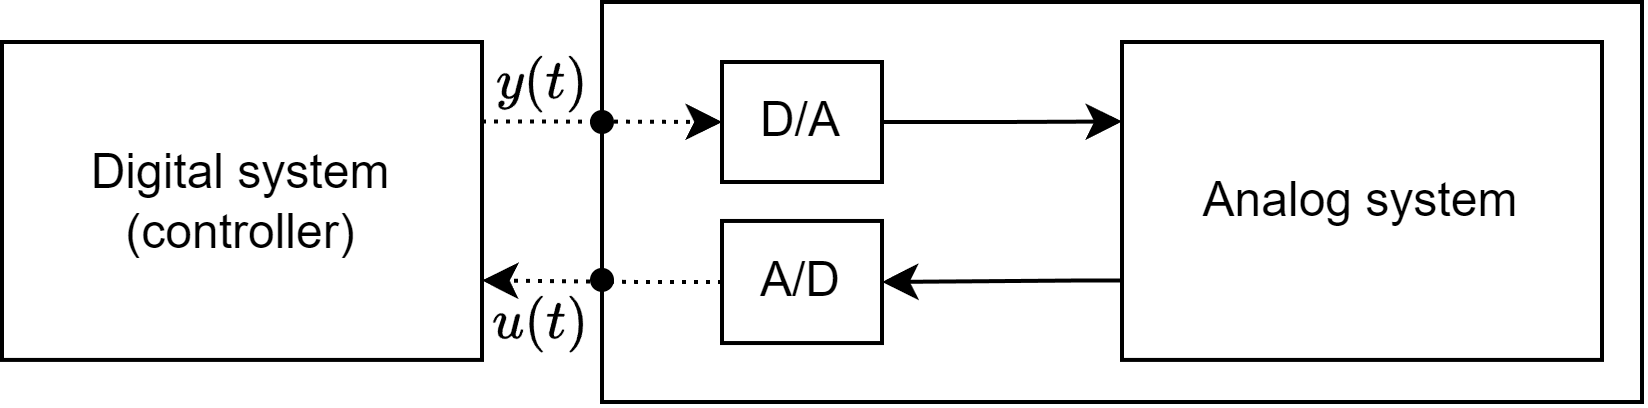
\includegraphics[width=0.5\linewidth]{images/sys.png}
    \caption{System}
\end{figure}
Beginning with a continuous model:
\[\mathcal{S}:\begin{cases} \dot{\mathbf{x}}=\mathbf{Ax}+\mathbf{Bu} \\ \mathbf{y}=\mathbf{Cx}+\mathbf{Du} \end{cases}\]
Assuming a sampling time of $\Delta T$: 
\[\mathcal{S}:\begin{cases} \mathbf{x}(t+1)=\mathbf{Fx}(t)+\mathbf{Gu}(t) \\ \mathbf{y}(t)=\mathbf{Hx}(t)+\mathbf{Du}(t) \end{cases}\]
The commonly used discretization method involves state space transformation:
\[\mathbf{F}=e^{\mathbf{A}\Delta T} \qquad \mathbf{G}=\int_0^{\delta T}e^{\mathbf{A}\delta}\mathbf{B} \,d\delta\qquad \mathbf{H}=\mathbf{C} \qquad \mathbf{D}=\mathbf{D}\]

\paragraph*{Poles discretization}
The poles of the continuous-time system are discretized into discrete time using the sampling transformation rule $\mathcal{Z}=e^{\mathcal{S}\Delta T}$, and so we have: 
\[\lambda_\mathbf{F}=e^{\lambda_\mathbf{A}\Delta T}\]
Here, $\lambda_F$ represents the eigenvalues of matrix $F$, and $\lambda_\mathbf{A}$ denotes the eigenvalues of matrix $\mathbf{A}$.

\paragraph*{Zeros discretization}
Beginning with the transfer function in continuous time:
\[G(s)=\dfrac{\text{polynomial in }s\text{ with }h \text{ zeros}}{\text{polynomial in }s\text{ with }n \text{ poles}}\]
Where $h<n$. 
In discrete time, we have:
\[G(z)=\dfrac{\text{polynomial in }z\text{ with }n-1 \text{ zeros}}{\text{polynomial in }z\text{ with }n \text{ poles}}\]
During the transformation of zeros from continuous to discrete time, $n-h-1$ new zeros are generated, known as hidden zeros.
Unfortunately, these hidden zeros do not adhere to the sampling rule and are typically non-minimum phase.